In this section we will illustrate the qualification process for the
openETCS tool chain.
As an example we will focus on the sample tool cahin depicted figure
\ref{fig:sample}

\begin{figure}[h]
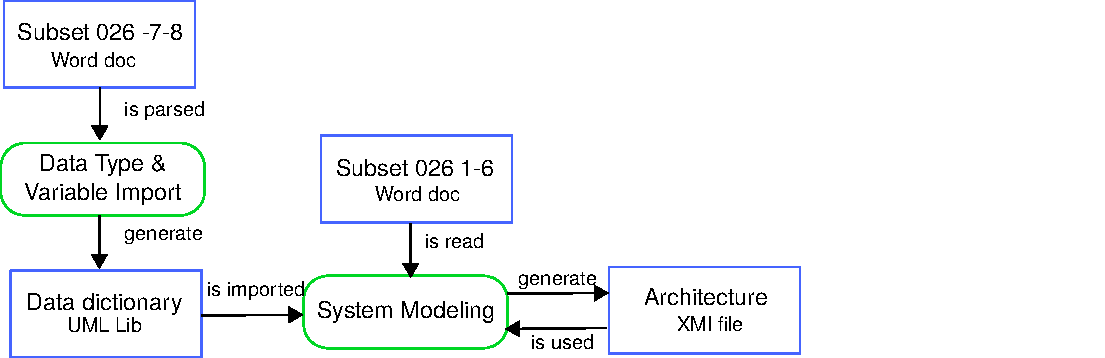
\includegraphics[width=\textwidth]{toolchainsample1}
\caption{\label{fig:sample} Tool chain sample} 
\end{figure}

\vskip 3em
\begin{figure}[h]
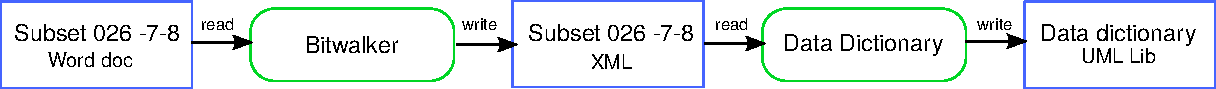
\includegraphics[width=\textwidth]{feature_analysis}
\caption{\label{fig:feature} Feature: Data type and Variable Import  }  
\end{figure}

The first tool chain : Create High-level Architecture I proposes to
create a high level view of the on board unit from the Subset 026
specification. It  contains two features : Data type and Variable
Import and the sytem modeling. Figure \ref{fig:feature} describes the
feature   ``Data type and Variable Import'' in more details.
The workflow is depicted figure \ref{fig:sample}. 

The tool chain analysis give us the following list of tool :
\begin{enumerate}
\item  Feature 1: Data type and Variable Import
\begin{itemize}
\item Tool 1: Bitwalker
\item Tool 2: Data Dictionary import
\end{itemize}
\item  Feature 2: System Modeling
\begin{itemize}
\item Tool 1: Papyrus Editor
\item Tool 2: Papyrus SysML Checker
\end{itemize}
\end{enumerate}

The following tables give the elements we could directly obtain from the
eclipse analysis that have to  be completed.

\begin{table}[htbp]
\centering
\caption{\label{tbl:datadict}Data dictionary  Information to be completed}
\begin{tabular}{|l|p{7cm}|}\hline
Tool Name: &Data Dictionary\\\hline
Version: &0.1.0 \\\hline
Tool License:& EUPL V1.1\\\hline
Tool Origin & Fraunhofer ESK, LAAS-CNRS \\
Tool Dependencies & - org.eclipse.ui \\
&-  org.eclipse.core.runtime\\
& - org.eclipse.emf.ecore\\
& - org.eclipse.papyrus.uml.extensionpoints \\ \hline
Description: & This feature contains the DataDictionary. The DataDictionary registers a UML model which contains data structure, variables and messages based on the ETCS System Requirements Specification (SRS). \\ \hline
Tool Class: & T3 \\\hline
\multicolumn{2}{|c|}{If T2/T3 Tools}\\\hline
Tool Justification & \\
 & \\ \hline
Manual Link and version & \\\hline
Artifact List link & \\\hline
Function List link& \\\hline
\multicolumn{2}{|c|}{If T3 Tools}\\\hline
Validation method& \\\hline
VnV activities report link&\\\hline
\end{tabular}
\end{table}

\begin{table}[htbp]
\centering
\caption{\label{tbl:bitwalker-info}Bitwalker Information to be completed}
\begin{tabular}{|l|p{5cm}|}\hline
Tool Name: & Bitwalker \\\hline
Version: & v1.0\\\hline
Tool License: & EUPL v1.1 \\\hline
Tool Origin: & Siemens for openETCS\\\hline
Tool Dependencies & None\\ \hline
Description: & Transform the word document chapter 7 and 8 to a XML file. \\ \hline
Tool Class: & T3 \\\hline
\multicolumn{2}{|c|}{If T2/T3 Tools}\\\hline
Tool Justification & \\
 & \\ \hline
Manual Link and version & \\\hline
Artifact List link & \\\hline
Function List link& see \ref{sec:bitwalker-example} \\\hline
\multicolumn{2}{|c|}{If T3 Tools}\\\hline
Validation method& \\\hline
VnV activities report link&\\\hline
\end{tabular}
\end{table}

\begin{table}[htbp]
\centering
\caption{\label{tbl:papyrus-info} Papyrus Editor Information to be completed}
\begin{tabular}{|l|p{5cm}|}\hline
Tool Name: & Papyrus Editor \\\hline
Version: &  0.10.1.v20130918 \\\hline
Tool License: & Eclipse \\\hline
Tool Origin: &  Eclipse Incubation (CEA)\\\hline
Tool Dependencies & \\
 & -\\
 & -\\ \hline
Description: & Papyrus is a modeling tool that allows us
    to model the high-level architecture of the OBU with SysML  \\ \hline
Tool Class: & T1\\\hline
\multicolumn{2}{|c|}{If T2/T3 Tools}\\\hline
Tool Justification &\\ \hline
Manual Link and version & \\\hline
Artifact List link & \\\hline
Function List link& \\\hline
\multicolumn{2}{|c|}{If T3 Tools}\\\hline
Validation method& \\\hline
VnV activities report link&\\\hline
\end{tabular}
\end{table}

\begin{table}[htbp]
\centering
\caption{\label{tbl:papyrusCheck-info} Papyrus Checker Information to be completed}
\begin{tabular}{|l|p{5cm}|}\hline
Tool Name: & Papyrus Checker \\\hline
Version: &  0.10.1.v20130918 \\\hline
Tool License: & Eclipse \\\hline
Tool Origin: &  Eclipse Incubation (CEA)\\\hline
Tool Dependencies & \\
 & -\\
 & -\\ \hline
Description: & Papyrus checker verifies the basics rules of SysML modeling. \\ \hline
Tool Class: & T2\\\hline
\multicolumn{2}{|c|}{If T2/T3 Tools}\\\hline
Tool Justification & To make import and export of the model the sysML
model should be consistent with SysML rules.\\ \hline
Manual Link and version & \\\hline
Artifact List link & \\\hline
Function List link& \\\hline
\multicolumn{2}{|c|}{If T3 Tools}\\\hline
Validation method& \\\hline
VnV activities report link&\\\hline
\end{tabular}
\end{table}

The artifact matrix for the tool chain matrix should look like
table \ref{tbl:example-artifacts}.
This table has beed pre-filled with the information available now,
this should also be completed during the qualification process.

\begin{table}[htbp]
\caption{\label{tbl:example-artifacts} List of  Artifacts Description\\ The
cells with ??? indicates unknown information\\ }
{\small
\begin{tabular}{|p{4em}|l|p{1.5cm}|l|p{5em}|p{1.8cm}|l|p{5em}|}\hline
Name & Format & Is read ? By who ?& Restrictions & Time stamp check? &Is
written ? By Who ?& Restrictions & Time Stamp produced ?\\\hline
Subset 026 chapt.7-8 & Word-docx & Bitwalker & none & no & no &
&\\\hline
Subset 026 chapt.7-8 & XML  & 
Data dictionary &  ??? & ??? & Bitwalker & ??? & ??? \\\hline
UML Library & XMI & Papyrus & Papyrus XMI & ??? & Data dictionary &
??? & ??? \\\hline 
Papyrus Model & XMI & Papyrus & Papyrus XMI & ??? & Papyrus &
 Papyrus XMI & ??? \\\hline 

\end{tabular}

}
\end{table}

